\chapter{Introduction}
\label{chapterlabel1}
\section{Charge Transport Regimes in Organic Semiconductors}
\subsection{Organic Semiconductors}
Conductive polymers were first discovered in 1977 by Shirakawa et al  \cite{chiang_electrical_1977, Shirakawa1977Jan} for which they were awarded the Nobel prize in Chemistry. Recently these materials have become ubiquitous in many technologies, such as in organic solar cells\cite{Kippelen2009}, organic field-effect transistors (OFET) \cite{Malachowski2010Jun} and organic light-emitting diodes (OLED) \cite{ThejoKalyani2012Jun}. While the other two technologies lag behind their inorganic counterparts, uptake of OLED screens is becoming increasingly popular especially in the smartphone and television market due to their flexibility, better colour reprsentation and lower energy consumption than conventional backlit LCD displays. In fact IHS markit's OLED market tracker predicts OLED to be the dominant technology in smartphone screens by 2020 \cite{IHSMarkit} \footnote{This is an online citation -Not sure whether I have cited correctly}. OLEDs have also found uses in lighting with their efficiency rivalling that of fluorescent tubes \cite{Reineke2009May, OLED_lighting}. Although, industry has made large strides in fabricating and using these materials the exact nature of the charge transport is still poorly understood. Conventional hopping and band theories break down in the regime of partial delocalisation of the charge carriers and atomistic simulations are required for a realistic picture.
\\\\
Typically charge carrier mobilities in `good' organic semiconductors (OSCs) fall between 1-10 cm$^2$ V$^{-1}$s$^{-1}$ \cite{yavuz_dichotomy_2017}. This is just beyond the range of hopping model validity ($\sim $ 1 cm$^2$ V$^{-1}$s$^{-1}$ ) and below that of band theory ($>$ 50 cm$^2$ V$^{-1}$s$^{-1}$ ). In this intermediate regime the charge carriers are typically not completely delocalised at the valence band edges (band regime) or localised to a single site/molecule (hopping regime) but delocalised over a few molecules. Without current analytic approaches being valid in this regime many computational approaches have been developed to investigate the underlying charge transport mechanisms \cite{oberhofer_charge_2017}.
\\\\
\subsection{Band-like Transport}
{\LARGE Band theory paragraph...}
\\\\
\subsection{Hopping-like Transport}
{\Large Need way more citations here -see Gajdos AOM paper it has lots of good references}
\\\\
Hopping theories assume the charge carrier is localised on one site and can hop from site to site in a series of discrete hops \cite{oberhofer_charge_2017}. There are various underlying mechanisms for this. For example, the presence of the charge carrier at a site can alter the nuclear geometry. The distorted nuclear geometry can make it harder for the charge carrier to move onto the next site, creating a metastable state and trapping the charge carrier. The deformation in the nuclear geometry is called a small polaron.
\\\\
{\LARGE Need a better connecting paragraph... Aim of the rest of this section is to lead on to the Born-Oppenhiemer approx}
\\\\
Polaronic hopping theories have been used to relative success and one of the key tools used in visualising this process (assuming harmonic response) are the Marcus Parabolas. These show how the free energy and reaction coordinates change after a charge transfer i.e. from initial to final diabatic states. The term `diabatic state' isn't well defined and can refer to different things in different formulations. In this work a diabatic state can be imagined as the charge carrier localised on a single molecule. This is discussed later in more detail in  \ref{sec:FOB-formalism}\\
\\
\begin{figure}[ht]
  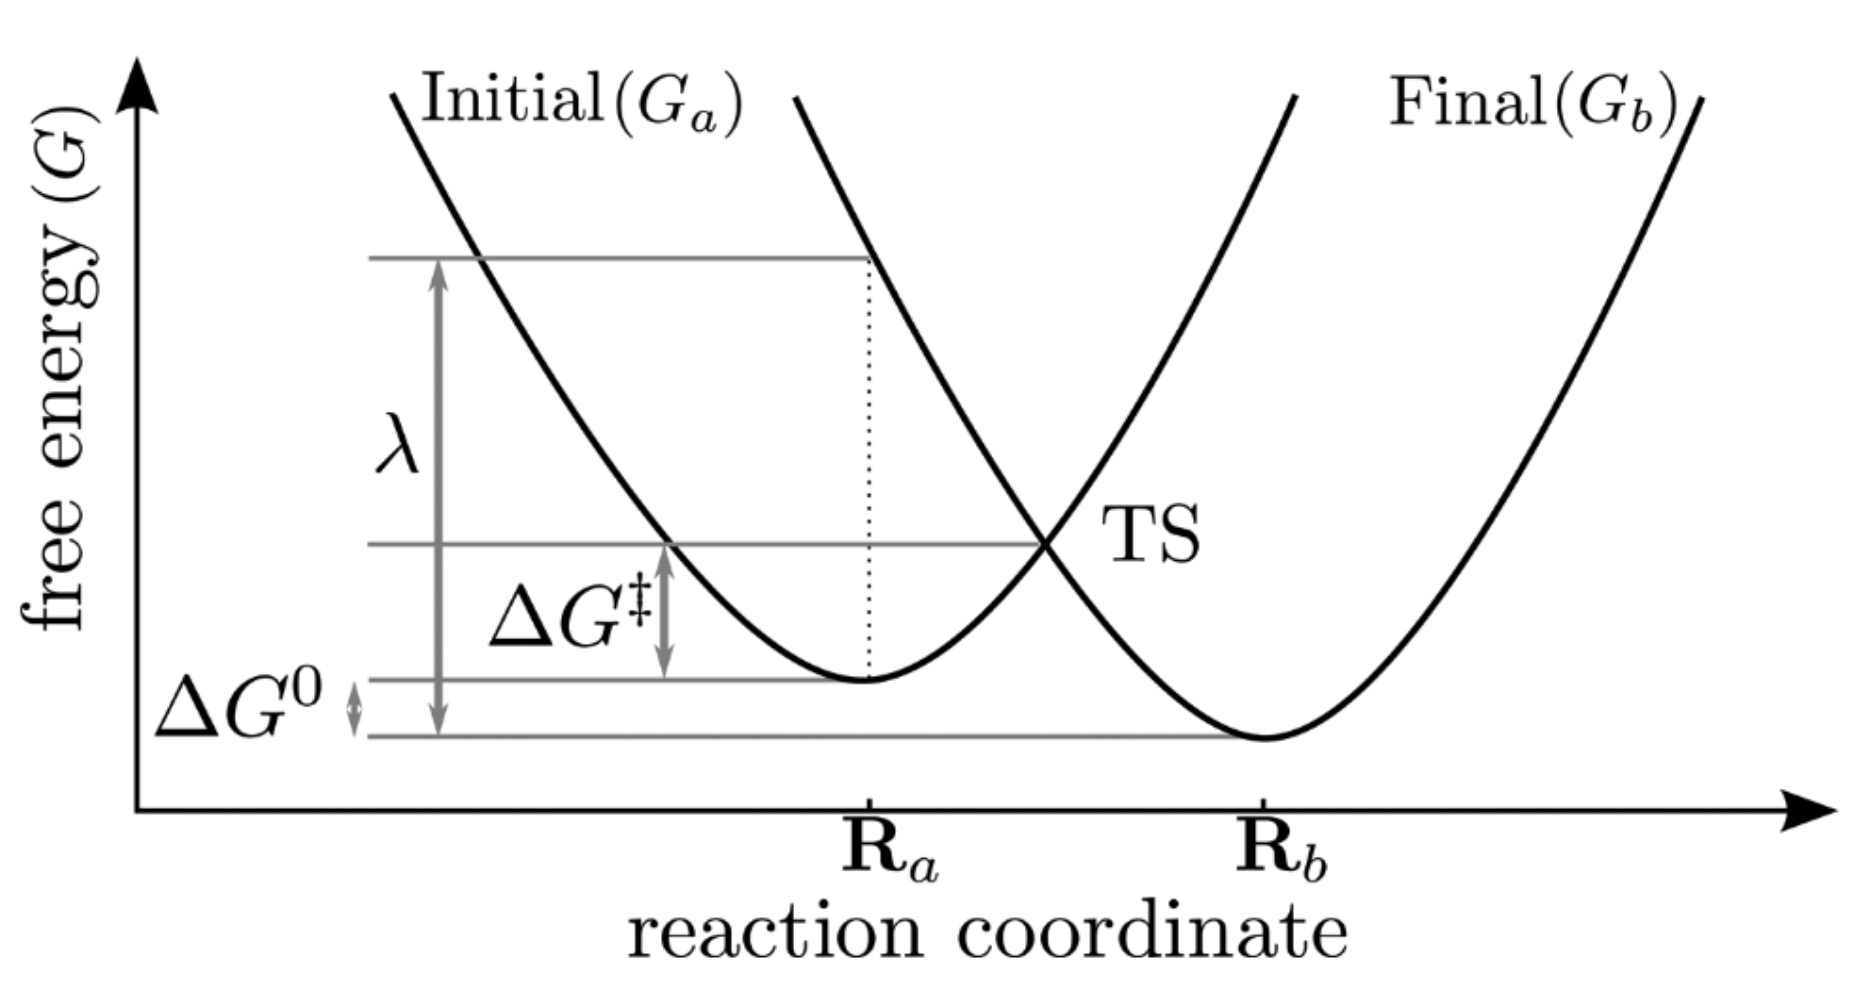
\includegraphics[width=\textwidth]{./img/diabatic_wells.png}
  \caption{Marcus parabolas depicting the relationship between the free energy in the system and the reaction coordinate at 0 electronic coupling. This figure was taken from Oberhofer et al \cite{oberhofer_charge_2017}}
  \label{fig:diab_wells}
\end{figure}
\\
Figure \ref{fig:diab_wells} above defines various important quantities for calculating the mobility in materials displaying hopping-like transport. The initial parabola describes the change in free energy with respect to the reaction coordinate for the initial state, for example when the charge is located on site 1. The final parabola describes the change in free energy when the charge is located on site 2 e.g. when the charge has relocated to site 2. The transition state (TS) is a point where the energies of the initial and final states are the same. This degenerate point is the only point at which the charge can move from the initial to final state as other points would result in a non-zero jump in energy between the 2 parabolas. The diabatic activation energy $\Delta G^{\ddagger}$ defines the energy required to get to this transition state from the minima of the initial parabola. The driving force $\Delta G^{0}$ is the difference in minima of the 2 parabolas, the reorganisation energy $\lambda$ defines the energy required to change the reaction coordinate from the final state minima to the initial state minima without changing electronic state.
\\\\
Figure \ref{fig:diab_wells} can change when there is a non-zero electronic coupling ($H_{ab}$) between diabatic states. This parameter increases the chance of moving between the initial and final diabatic states by lowering the diabatic activation energy i.e. the energy required to transition from state 1 to 2. This is visualised in figure \ref{fig:adiab_wells}
\begin{figure}[ht]
  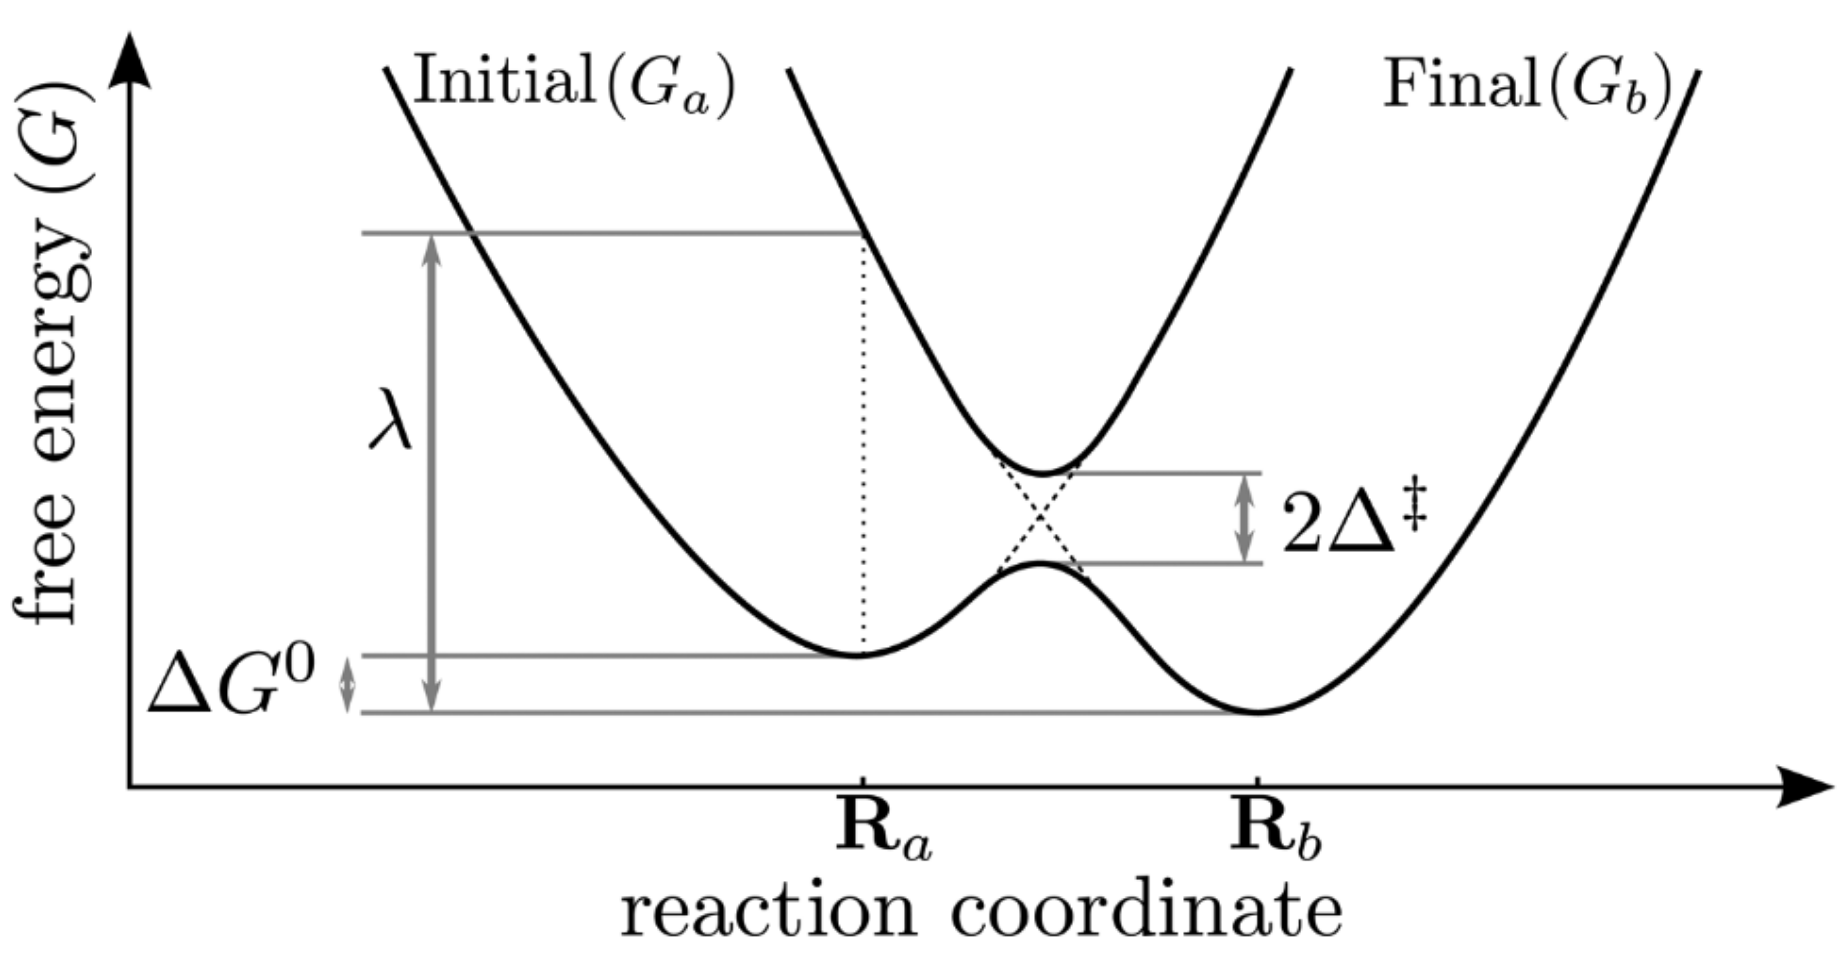
\includegraphics[width=\textwidth]{./img/adiabatic_wells.png}
  \caption{Graph depicting the change in free energy for a change in reaction coordinate for non-zero electronic coupling. Adapted from \cite{oberhofer_charge_2017}}
  \label{fig:adiab_wells}
\end{figure}
In figure \ref{fig:adiab_wells} above the diabatic activation energy has be lowered to $\Delta G^{\dagger} = \Delta G^{\ddagger} - H_{ab}$ making it easier for charge carriers to transition between diabatic states. In our formalism this means it is easier for charge carriers to move between sites i.e. delocalise. We see also that instead of being described totally by 2 parabolas there are 2 new adiabatic potential energy surfaces arising -the ground and excited state. The amount that these new potential energy surfaces diverge from the diabatic wells is dependent on an adiabaticity factor which is proportional to the ratio between the electronic coupling, $H_{ab}$, and the re-organisation energy, $\lambda$. This has been discussed in detail in multiple papers \cite{oberhofer_charge_2017, spencer_fob-sh:_2016, spencer_confronting_2016,   Gajdos2013Mar} .
\\\\
In fact for systems with couplings larger than $H_{ab} > \frac{3}{8} \lambda$ the diabatic activation energy vanishes completely \cite{Gajdos2013Mar}, meaning that there is no energy cost in transitioning between diabatic states. Beyond this regime hopping theories cannot be accurately applied. Unfortunately, at room temperatures thermal flucuations means the mean free path of the charge carriers is comparable to the intermolecular spacing. As such band theories too are inapplicable
\cite{oberhofer_charge_2017, gajdos_ultrafast_2014, Gershenson2006Sep}. Much beyond this regime the energy cost to transition to higher adiabatic potential energy surfaces becomes prohibitively high and the system travels on a single state. In these situations the Born-Oppenhiemer approximation is valid. However, in this work I will be looking into the regime in between the band and hopping-like transport where we currently don't have  analytical theories to describe charge transport. For this I will be using non-adiabatic atomistic simulations, namely a technique called CTMQC.
\section{Atomisitc Simulations of Nonadiabatic Processes}
In simulating processes involving electronic transfers a key approximation used in conventional molecular dynamics (MD) breaks down. That is the Born-Oppenheimer or adiabatic approximation \cite{john_c._tully_nonadiabatic_nodate}. This approximation relies on the fact that nuclei are more massive than electrons and are approximately stationary with respect to electron movement (need ref). This results in nuclear evolution that is governed by a single, adiabatic, potential energy surface. However, in many interesting processes, such as electron transfer, non-radiative decay and photochemical processes, electronic transitions between adiabatic potential energy surfaces occur (need ref). Simulating these processes requires non-adiabatic molecular dynamics (NAMD) techniques to be developed to correctly capture dynamical properties.
\\\\
There have been many techniques proposed for use in NAMD such as the quantum classical Louiville equation (need ref), multiple spawning (need ref) or nonadiabatic Bohmian dynamics (need ref) \footnote{See first Frederica paper} . However, two of the most popular are trajectory surface hopping (need ref) and mean-field approaches (need ref). This is probably due to their relative simplicity to implement (need ref), efficiency for large systems (need ref) and proven efficacy in a wide variety of situations (need ref). In all of these approaches the general aim is to treat as much of the system as possible with (computionally cheaper) classical mechanics. While handling all necessary parts with quantum mechanics \cite{Coker1995Jan}. In Surface Hopping, Ehrenfest and CTMQC one treats the nuclear subsystem classically and the electronic one quantum mechanically. The nuclei are propagated using a velocity verlet algorithm according to Newton's laws. The electrons are propagated using a fourth order Runge Kutta algorithm according to the time-dependent Schr\"odinger equation. This is normally expanded as a linear combination of adiabatic or diabatic states. The nuclei and electrons can also interact. Taking account of this interaction is where these different atomistic simulation techniques differ.
\subsection{FOB Formalism \label{sec:FOB-formalism}}
The effect of the nuclei on the electrons is normally handled via the Hamiltonian. This is dependent on nuclear positions and is in turn used in the Schr\"odinger equation to propagate the electron dynamics. Often the construction of the Hamiltonian is carried out using density function theory (DFT). However, for large, dynamic systems this becomes too computationally expensive and a different technique would have to be used. In this work I will rely on an Analytical Overlap Method (AOM) \cite{gajdos_ultrafast_2014} to calculate the off-diagonal elements of the Hamiltonian and the diagonal elements will be calculated via a forcefield.
\subsubsection{AOM}
AOM assumes that the off-diagonal elements of the Hamiltonian are proportional to the off-diagonal elements of the overlap matrix between 2 singly occupied molecular orbitals (SOMO). For $\pi$-conjugated systems,
\subsection{Surface Hopping and Ehrenfest Dynamics}
{\LARGE How surface hopping and ehrenfest alter the potential energy surface to affect the nuclear dynamics}
\\\\
\section{CTMQC \label{intro:CTMQC}}
CTMQC comes from taking the semi-classical limit of an exact factorisation of the molecular wavefunction into its constituent electronic and nuclear components \cite{abedi_exact_2010}. Where the electronic component is parametrically dependent on the nuclear coordinates, $\textbf{R}$. This is shown below in eq \eqref{eq:exact_fact} where $\chi$ is the nuclear wavefunction and $\Phi$ is the electronic one.
\begin{equation}
 \Psi(\textbf{R}, \textbf{r}, t) = \Phi_{\textbf{R}}(\textbf{r}, t) \chi(\textbf{R}, t)
 \label{eq:exact_fact}
 \end{equation}
In the above equation (and throughout this report) I will denote nuclear coordinates and electronic coordinates $R$ and $r$ respectively. The nuclear and electronic wavefunctions then obey separate, but coupled, time-dependent schr\"odinger equations for spatial and temporal evolution. This representation has proven to be useful in furthering understanding through exact solutions of small toy-model systems (need ref \footnote{see deconstruction paper}). However, in this report I will be focussing on the semi-classical limit of these equations (CTMQC) and give some early results of a combination of this and the AOM method explained previously in section \ref{sec:FOB-formalism}.
The equations for the evolution of the electronic and nuclear wavefunctions in the exact factorisation \cite{abedi_exact_2010} are given below:
\begin{align}
  i\hbar \frac{\delta}{\delta t} \Phi_{\textbf{R}}(\textbf{r}, t) &= \left( \hat{H}_{BO} + \hat{U}_{en}\left[ \Phi_{\textbf{R}}, \chi\right] - \epsilon(\textbf{R}, t) \right) \Phi_{\textbf{R}} (\textbf{r}, t)
  \label{eq:electronic_exact}
\\
i\hbar \frac{\delta}{\delta t} \chi (\textbf{R}, t) &= \left( \sum_{\nu = 1}^{N_{n}} \frac{[-i\hbar\nabla_{\nu} + \textbf{A}_{\nu}(\textbf{R}, t)]^2}{2 M_{\nu}} + \epsilon(\textbf{R}, t)\right) \chi (\textbf{R}, t)
  \label{eq:nuclear_exact}
\end{align}
Where $\hat{H}_{BO}$ is the Born-Oppenheimer Hamiltonian, that is $\hat{T}_{e} + \hat{W}_{ee} + \hat{W}_{nn} + \hat{V}_{en}$. Where $\hat{T}_{e}$ is the electronic kinetic energy operator, $\hat{W}_{ee/nn}$ is the electron-electron/nuclei-nuclei interation and $V_{en}$ is the electronic-nuclear potential.
\\\\
The $\hat{U}_{en}$ is an electronic-nuclear coupling operator (ENCO). This is defined as $  \hat{U}_{en}[\Phi_{\textbf{R}}, \chi] = \sum_{\nu=1}^{N_{nuc}} \frac{1}{M_{\nu}} \left[ \frac{\left[-i \hbar \nabla_{\nu} - \textbf{A}_{\nu}(\textbf{R}, t) \right]^2}{2} + \left( \left. \left. \frac{-i\hbar \nabla_{\nu} \chi}{\chi} + \textbf{A}_{\nu}(\textbf{R, t})\right)\right( -i\hbar\nabla_{\nu} - \textbf{A}_{\nu}(\textbf{R}, t)\right) \right]   $.
Where the $\textbf{A}_{\nu}$ is a time-dependent vector potential (TDVP), given by $\left\langle \Phi_{\textbf{R}}(t) \right\vert \left. - i \hbar \nabla_{\nu} \Phi_{\textbf{R}} \right\rangle_{\textbf{r}}$ and $M_{\nu}$ is the mass of nuclei $\nu$.
Finally $\epsilon(\textbf{R}, t)$ is a time-dependent scalar potential energy surface (TDPES), given by $\langle \Phi_{\textbf{R}}(t) \vert \hat{H}_{BO} + \hat{U}_{en}^{coup} - i\hbar \frac{\delta}{\delta t} \vert \Phi_{\textbf{R}}(t) \rangle_{\textbf{r}}$.
\begin{wrapfigure}{r}{0.45 \textwidth}
  \includegraphics[width=0.7\textwidth]{./img/nuclear_splitting_TDPES.png}
  \caption{A demonstration of how the TDPES can cause the splitting of the nuclear wavepacket in non-adiabatic regions. The red line represents the TDPES and the blue is the nuclear density. Adapted from \cite{agostini_exact_2015} \label{fig:step_TDPES}}
\end{wrapfigure}
\\
The effects of these latter terms (the TDPES, TDVP and the ENCO) have been investigated in multiple works \cite{agostini_semiclassical_2015, agostini_exact_2015, agostini_mixed_2013, abedi_dynamical_2013, Min2014Dec}. The TDPES and TDVP are both responsible for the evolution of the system
\cite{agostini_semiclassical_2015}.  The TDPES provides exact classical forces on the nuclei. In fact, an alternative independent-trajectory semi-classical scheme has been investigated using these exact forces \cite{agostini_exact_2015}. This found the TDPES is responsible for the splitting of the nuclear wavepacket in regions of high non-adiabaticity by taking the shape of a step function. This is demonstrated in figure \ref{fig:step_TDPES}.
\\\\


\newpage



\begin{itemize}
\item Brief introduction to NAMD.
\begin{itemize}
\item \st{Why isn't normal MD good enough?}
\item \st{What sort of processes need NAMD to simulate them?}
\item Characteristics of NAMD -Trivial Crossings, avoided crossings.
\item Give current standard methods and their advantages/disadvantages
\end{itemize}
\item Briefly explain the AOM method.
\begin{itemize}
\item How it works - The analytic off-diagonal elements of hamiltonian (Spencer -both)
\item What the alternatives are (Gajdos paper)
\item Why this is preferable (Gajdos)
\item What are the limitations
\end{itemize}
\item Explain CTMQC
\begin{itemize}
\item Intro -It was derived from exact factorisation (maybe put derivation in appendix)
\item Give the equations. -Ehrenfest + QM term
\item How does it compare to other techniques -decoherence, first principles
\item Why combine it with FOB-CTMQC? -Expensive DFT etc...
\item What sort of systems will I be looking at? Charge transfer in organic semiconductors -1D and 2D systems
\end{itemize}

\end{itemize}
Then Results
